\begin{figure}[H]
    \centering
    \begin{subfigure}[b]{0.15\textwidth}
        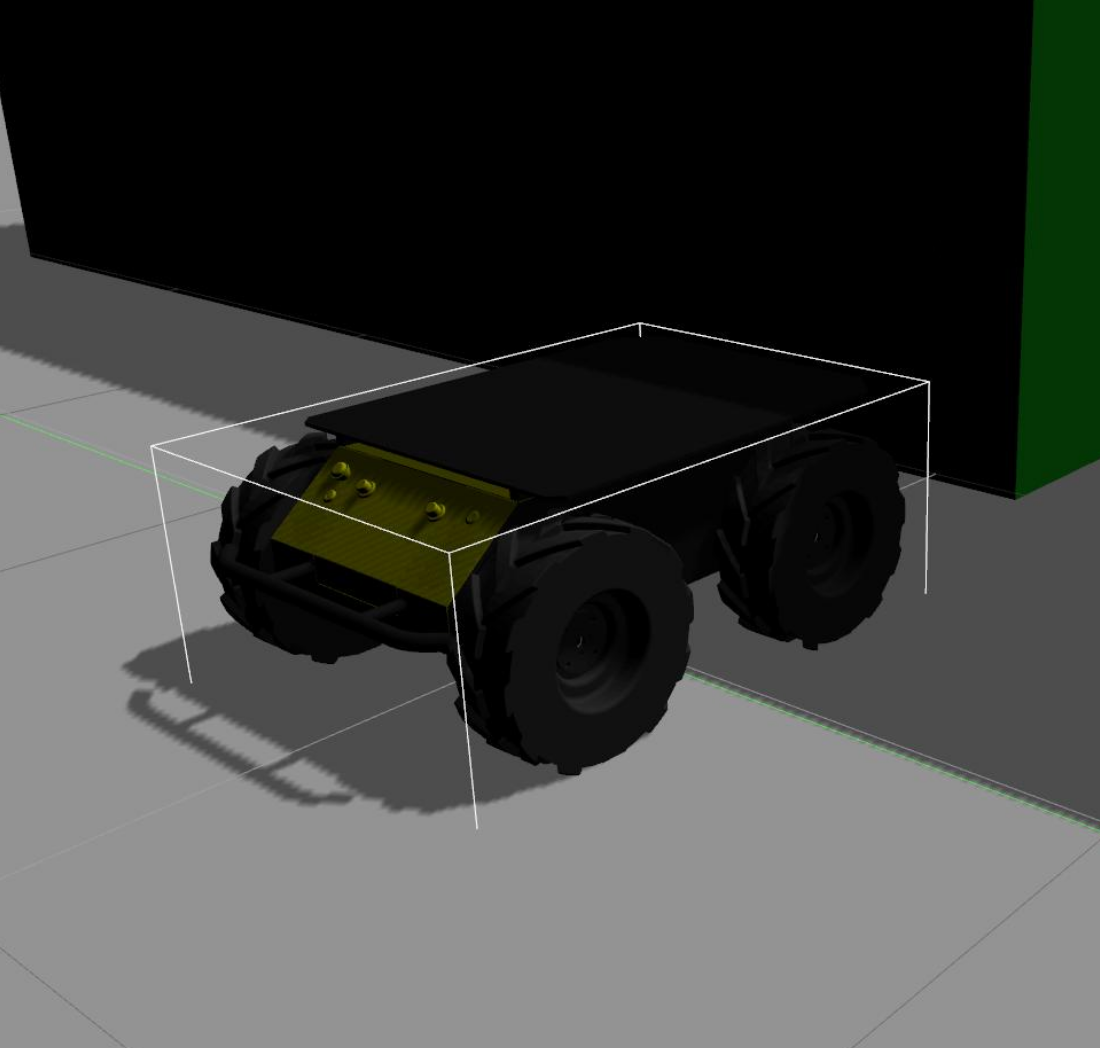
\includegraphics[width=\textwidth]{bot1}
        \caption{Husky bot}
        \label{fig:bot1}
    \end{subfigure}
    \begin{subfigure}[b]{0.15\textwidth}
        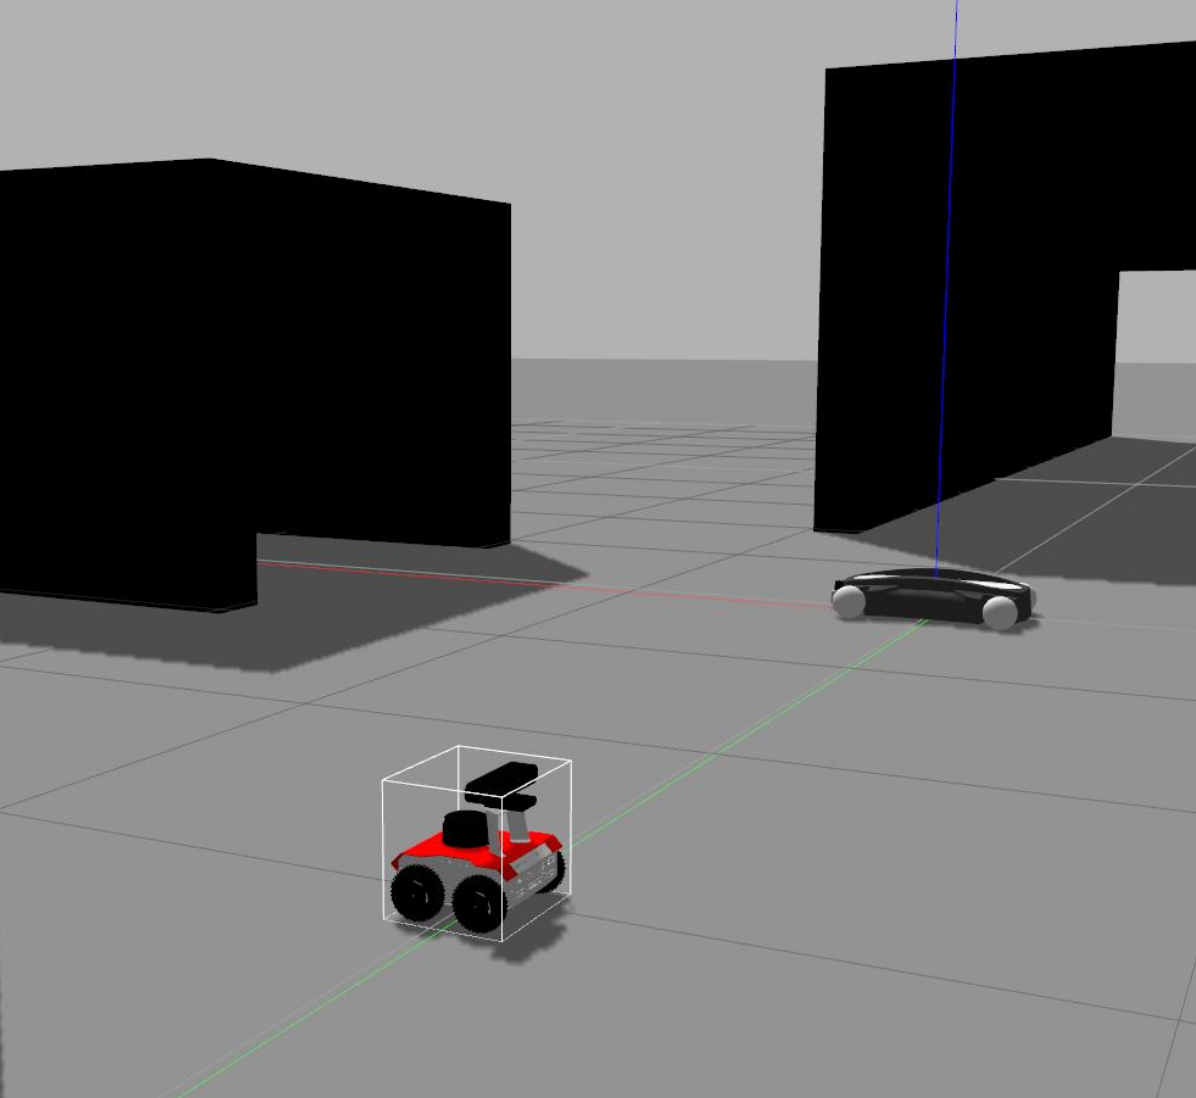
\includegraphics[width=\textwidth]{bot2}
        \caption{Rosbot}
        \label{fig:bot2}
    \end{subfigure}
    \begin{subfigure}[b]{0.15\textwidth}
        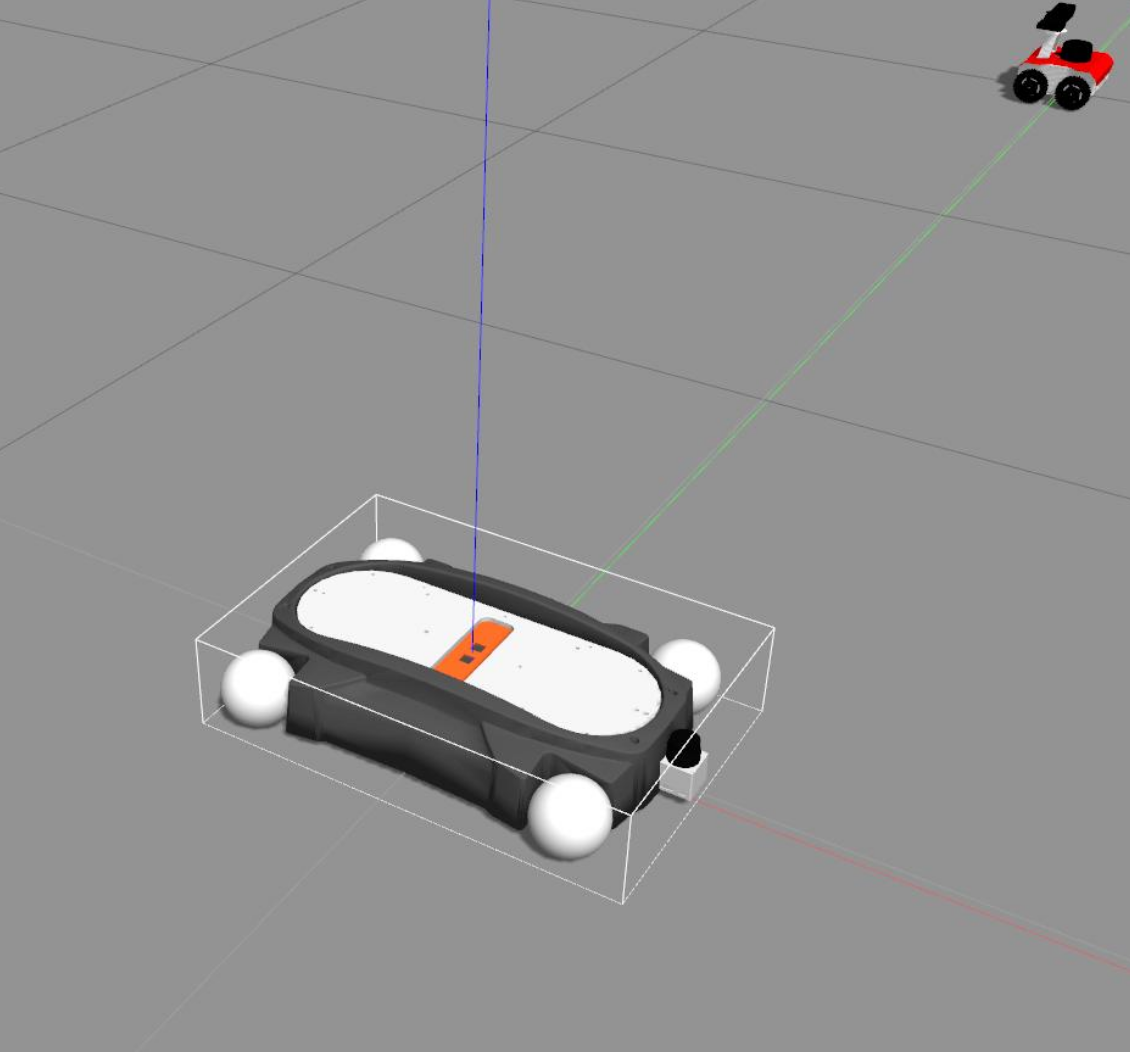
\includegraphics[width=\textwidth]{bot3}
        \caption{Youbot}
        \label{fig:bot3}
    \end{subfigure}
    \label{fig:robots}
    \caption{Three commonly used robots with very different shapes, sizes, and capabilities.}\label{fig:bots}
\end{figure}

The study of multi-robot systems and autonomous swarms is becoming more and more of a hot topic in
the world today. Being able to parallelize a large task or simply cover more ground, these systems
have the capability to perform a lot of interesting and tedious tasks to the common individual.
More often than not, these applications are inherently homogeneous, meaning each robot is the same
as this could be cheaper and build in more of a fault tolerant attitude. One downside to homogeneity
in the context of multi-robot systems is that the overall system would be limited based on the capabilities
of that specific type of robot. This brings to mind the idea of utilizing heterogeneous robots to accomplish
singular tasks. A lot of research has gone into
heterogeneous multi-robot systems in the past few years, but a common trend
amongst most of them is that the model is built for the specific platforms
that are to be used. For instance if a researcher utilized a UGV and UAV as their
heterogeneity agent makeup. This proposed research aims to tackle that problem and
to encourage interest and experimentation in the field of heterogeneous multi-robot systems.
Upon iterations, this research will ultimately be meant to provide the groundwork
for a heterogeneous model that allows for the insertion of a robots with different
skill sets with the purpose of enhancing the overall capability of the system.
This framework would allow for a variety of models to be built on top of it,
with a variety of hardware. Researchers wanting to build a specific system
could allocate funds and resources to build each member to accomplish a portion
of the overall task, possibly allowing for more cost efficiency and remove
unnecessary redundancy. The main challenge in this research will be finding
the optimal way to reassign tasks and have a variety of systems work together to accomplish
a global task. With primary informatic clashes would occur at the sensor level with varying sensor models as
well as at the control level relating to movement capabilities. What was not necessarily
expected out of this research was a structured and
easy to understand testing package for heterogeneous systems developed in ROS and simulated with GAZEBO \cite{ROS} .
Due to encountered limitations with initially chosen software and technology, the development
of this framework is necessary to fully test this concept before taking the step towards hardware.
